% Shared typography and palette for the research schematics.
\documentclass[tikz,border=9pt]{standalone}
\usepackage[T1]{fontenc}
\usepackage{lmodern}
\usetikzlibrary{arrows.meta,calc,positioning,backgrounds}
\renewcommand{\familydefault}{\sfdefault}
\hyphenpenalty=10000
\exhyphenpenalty=10000
\definecolor{Ink}{HTML}{263D4A}
\definecolor{Muted}{HTML}{536774}
\definecolor{Blue}{HTML}{24678E}
\definecolor{Teal}{HTML}{0D6B6E}
\definecolor{Green}{HTML}{26734D}
\definecolor{Gold}{HTML}{87641A}
\definecolor{PaleBlue}{HTML}{EDF4FA}
\definecolor{PaleTeal}{HTML}{ECF6F5}
\definecolor{PaleGreen}{HTML}{EFF6F0}
\definecolor{PaleGold}{HTML}{FAF5E9}
\definecolor{PaleGray}{HTML}{F2F5F6}
\tikzset{
  every node/.style={text=Ink,font=\sffamily\fontsize{11}{14}\selectfont},
  panel/.style={draw=#1!65,fill=#1!5,line width=.7pt,rounded corners=5pt,
    minimum width=5.7cm,minimum height=3.4cm,text width=4.95cm,
    inner sep=10pt,align=left,anchor=north west},
  flow/.style={-{Stealth[length=5pt,width=5pt]},draw=Muted,line width=1pt,
    shorten <=4pt,shorten >=4pt},
  note/.style={text width=11.8cm,align=left,font=\sffamily\fontsize{10}{13}\selectfont,
    text=Muted,anchor=north west},
}
\newcommand{\heading}[2]{
  \node[anchor=north west,text width=12.4cm,font=\sffamily\bfseries\fontsize{21}{25}\selectfont]
    at (0,1.9) {#1};
  \node[note] at (0,.85) {#2};
}
\newcommand{\panel}[6]{
  \node[panel=#4] (#1) at (#2,#3)
    {{\color{#4}\bfseries\fontsize{13}{16}\selectfont #5}\\[5pt]#6};
}
\newcommand{\fourflow}{
  \draw[flow] (a.east) -- (b.west);
  \draw[flow] (b.south) -- (c.north);
  \draw[flow] (c.west) -- (d.east);
}
\newcommand{\bottomnote}[1]{\node[note] at (0,-7.75) {#1};}
% Suppress volatile PDF metadata; SOURCE_DATE_EPOCH is also set by the builder.
\ifdefined\pdfinfoomitdate\pdfinfoomitdate=1\fi
\ifdefined\pdftrailerid\pdftrailerid{}\fi
\ifdefined\pdfsuppressptexinfo\pdfsuppressptexinfo=15\fi

\begin{document}
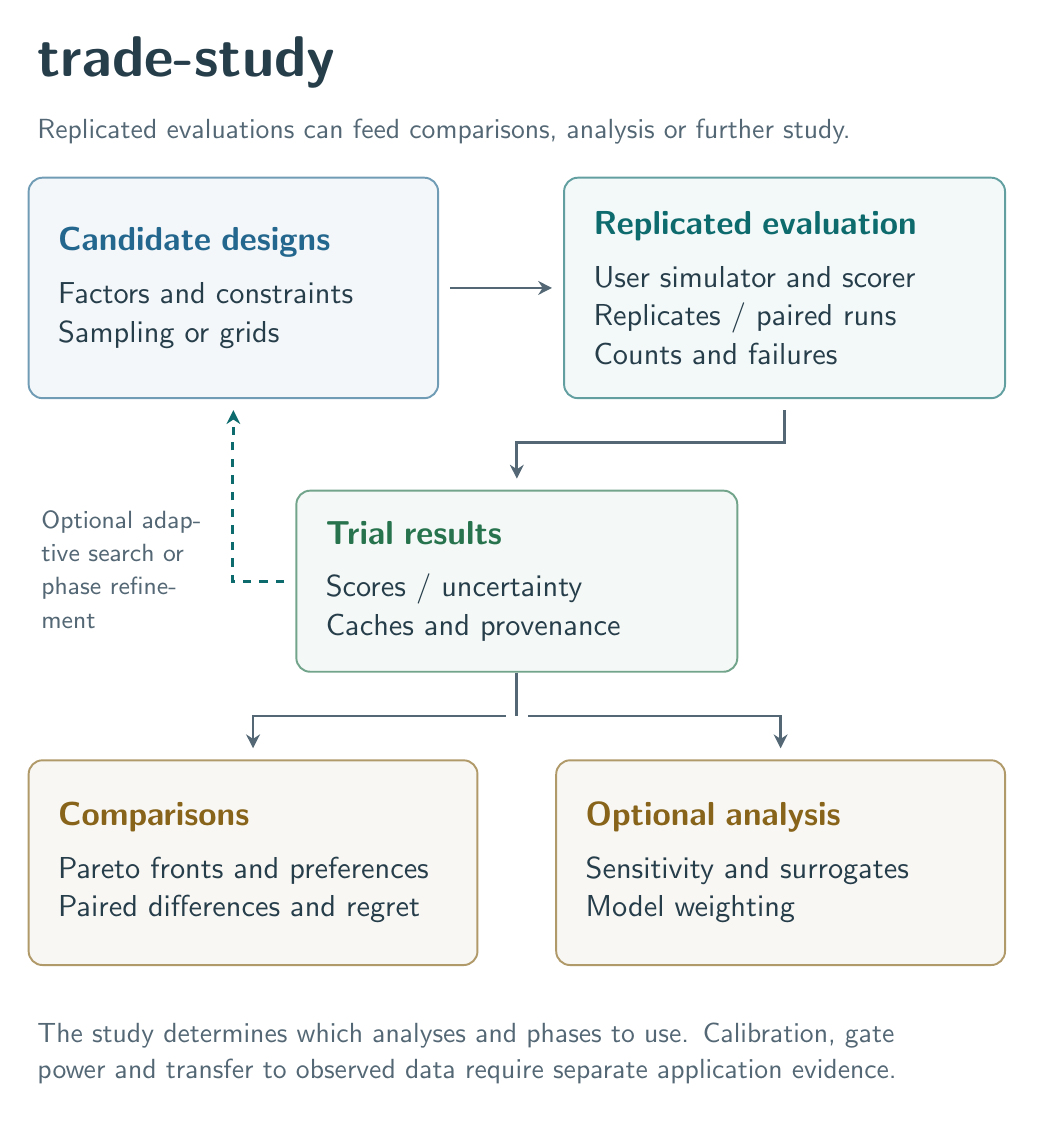
\begin{tikzpicture}
\heading{trade-study}{Replicated evaluations can feed comparisons, analysis or further study.}
\node[panel=Blue,minimum width=5.2cm,text width=4.45cm,minimum height=2.8cm] (designs) at (0,0)
  {{\color{Blue}\bfseries\large Candidate designs}\\[5pt]Factors and constraints\\Sampling or grids};
\node[panel=Teal,minimum width=5.6cm,text width=4.85cm,minimum height=2.8cm] (evaluation) at (6.8,0)
  {{\color{Teal}\bfseries\large Replicated evaluation}\\[5pt]User simulator and scorer\\Replicates / paired runs\\Counts and failures};
\node[panel=Green,minimum width=5.6cm,text width=4.85cm,minimum height=2.3cm] (results) at ($(evaluation.south -| designs.west)+(3.4,-1.15)$)
  {{\color{Green}\bfseries\large Trial results}\\[5pt]Scores / uncertainty\\Caches and provenance};
\node[panel=Gold,minimum width=5.7cm,text width=4.95cm,minimum height=2.6cm] (comparison) at ($(results.south -| designs.west)+(0,-1.1)$)
  {{\color{Gold}\bfseries\large Comparisons}\\[5pt]Pareto fronts and preferences\\Paired differences and regret};
\node[panel=Gold,minimum width=5.7cm,text width=4.95cm,minimum height=2.6cm] (analysis) at ($(comparison.north west)+(6.7,0)$)
  {{\color{Gold}\bfseries\large Optional analysis}\\[5pt]Sensitivity and surrogates\\Model weighting};
\draw[flow] (designs.east) -- (evaluation.west);
\draw[flow] (evaluation.south) -- ++(0,-.55) -| (results.north);
\coordinate (branches) at ($(results.south)+(0,-.55)$);
\draw[draw=Muted,line width=1pt] (results.south) -- (branches);
\draw[flow] (branches) -| (comparison.north);
\draw[flow] (branches) -| (analysis.north);
\draw[flow,dashed,draw=Teal] (results.west) -- ++(-.8,0) |- ($(designs.south)+(0,-.5)$) -- (designs.south);
\node[note,text width=2.2cm,font=\sffamily\fontsize{9}{12}\selectfont] at ($(results.north -| designs.west)+(.05,-.15)$) {Optional adaptive search or phase refinement};
\node[note] at ($(comparison.south west)+(0,-.6)$) {The study determines which analyses and phases to use. Calibration, gate power and transfer to observed data require separate application evidence.};
\end{tikzpicture}
\end{document}
